\documentclass[border=8pt]{standalone}
\usepackage{tikz}
\usetikzlibrary{arrows.meta, positioning, calc}

\begin{document}
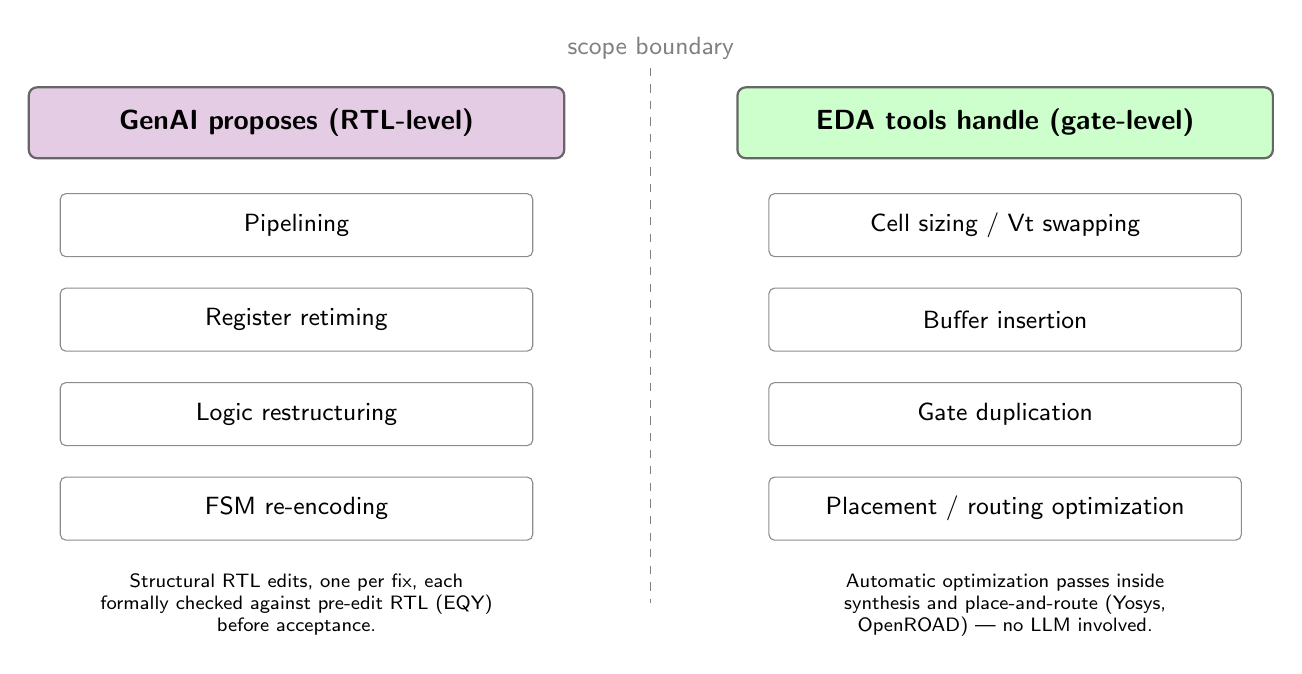
\begin{tikzpicture}[
  font=\sffamily,
  head/.style={rectangle, rounded corners=3pt, draw=black!60, thick, fill=#1,
               minimum height=9mm, minimum width=68mm, align=center, font=\sffamily\bfseries},
  item/.style={rectangle, rounded corners=2pt, draw=black!45, thin, fill=white,
               minimum height=8mm, minimum width=60mm, align=center, font=\sffamily\small},
  sub/.style={font=\sffamily\scriptsize, text width=60mm, align=center},
]

% ---- Left column: GenAI / RTL-level ----
\node[head=violet!20] (hL) at (0,0) {GenAI proposes (RTL-level)};
\node[item] (l1) at (0,-1.3) {Pipelining};
\node[item] (l2) at (0,-2.5) {Register retiming};
\node[item] (l3) at (0,-3.7) {Logic restructuring};
\node[item] (l4) at (0,-4.9) {FSM re-encoding};
\node[sub, below=3mm of l4] {Structural RTL edits, one per fix, each\\formally checked against pre-edit RTL (EQY)\\before acceptance.};

% ---- Right column: EDA tools / gate-level ----
\node[head=green!20] (hR) at (9,0) {EDA tools handle (gate-level)};
\node[item] (r1) at (9,-1.3) {Cell sizing / Vt swapping};
\node[item] (r2) at (9,-2.5) {Buffer insertion};
\node[item] (r3) at (9,-3.7) {Gate duplication};
\node[item] (r4) at (9,-4.9) {Placement / routing optimization};
\node[sub, below=3mm of r4] {Automatic optimization passes inside\\synthesis and place-and-route (Yosys,\\OpenROAD) --- no LLM involved.};

\draw[dashed, gray] (4.5,0.7) -- (4.5,-6.1);
\node[font=\sffamily\small, gray] at (4.5,0.95) {scope boundary};

\end{tikzpicture}
\end{document}
